%This is chapter 3
%%=========================================
\chapter[Method]{Materials and methods}

%In this final chapter you should sum up what you have done and which results you have got. You should also discuss your findings, and give recommendations for further work.

%%=========================================

\section{Project Organisation}
The group consists of ...
Meetings ....

\section{Working methodology}
\section{Scrum}
Even though i am alone, i have tried to adapt the scrum methodology.

\section{GitFlow}

\section{Requirements sepcification}
Acceptance criteria - custom field in Jira.
Specially for the voxelisation algorithm.

\section{Tools and libraries}

\section{Semantic versioning}

\subsection{JavaScript version}
ES6 - needs to be transpiled with Babel.

\subsection{Third party libraries}
Why did i use them???
list up like:
- xxx because ...
- xxx provides ...
Elaborate some on three.js


\subsection{GitHub Actions}
Why? How did i use it?

\section{Debugging and metrics}
how did i provide this?

\section{Graphix}
three-voxel-loader


\section{Voxelization}
The voxelization algorithm is mainly based on picking. More specifically, raycasting. ..........

Alternatively to raycasting, one could make use of color picking. This is in principle significantly quicker than normal raycasting since it is computed on the GPU. One could render a "heightmap" from each side of the 3D model. Each pixel in the heightmaps could then be looped over, mapping the pixel color back to the face's location in space, representing a filled voxel. Even though effective, it has a severe downside. No hidden or internal structures would be detected with this sort of system. Raycasting is therefore the obvious choise, even thoug it is CPU bound.

\subsection{Raycasting}
The raycasting is supplied by three.js library. The library provides a thoughourly tested and accurate raycasting solution.

The raycasting is demonstrated in figure \ref{fig:raycasting-intersections-example}. A ray is directed towards an object. If it intersects a face

\begin{figure}[h]
    \centering
    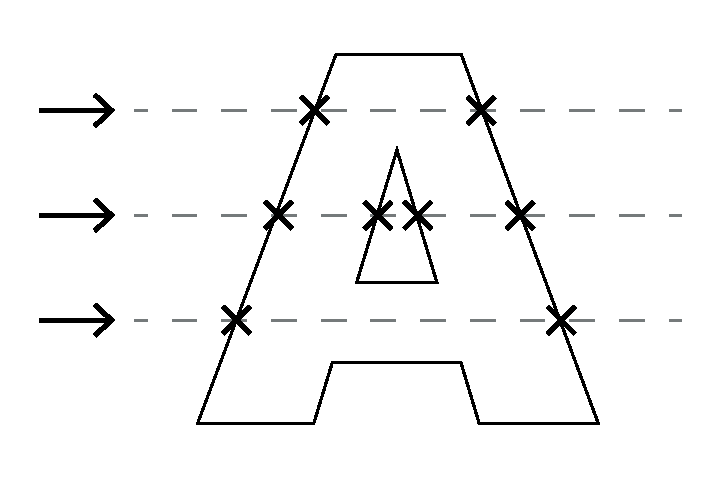
\includegraphics[scale=0.8]{sections/methodology/figures/raycast-intersections}
    \caption{Raycasting intersections example.}
    \label{fig:raycasting-intersections-example}
\end{figure}


Asd

\subsection{Algorithm}
Asd

\subsection{Shell voxelization}
Asd

\subsection{Solid voxelization}
\colorbox{RubineRed}{Maybe more discussion or result related?}
The solid voxelisation, or filled voxelisation, is achieved by interpreting the first raycast intersect as the surface of the object. From this point will everything be considered "inside" the object. When a second intersect is detected, the state is changed to be "outside" the object. A new hit would indicate "inside", and so on. This works verry well with a watertight (\colorbox{RubineRed}{edges are manifolded?}) 3D model, as can be seen from figure \ref{fig:filling-non-watertight-model}. However, when trying to fill an object which is not watertight, this can result in severe inaccuracies. This can be seen in figure \ref{fig:filling-watertight-model}

\begin{figure}[h]
    \centering
    \begin{subfigure}[b]{0.45\textwidth}
        \centering
        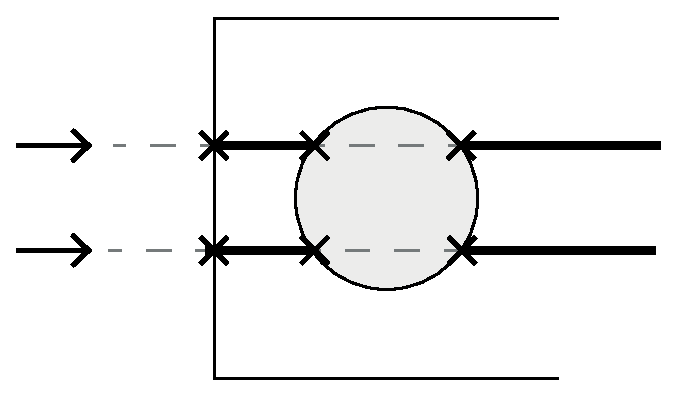
\includegraphics[width=\textwidth]{sections/methodology/figures/solid-non-watertight}
        \caption{Non-watertight 3D model cross section.}
        \label{fig:filling-non-watertight-model}
    \end{subfigure}
    \hfill
    \begin{subfigure}[b]{0.45\textwidth}
        \centering
        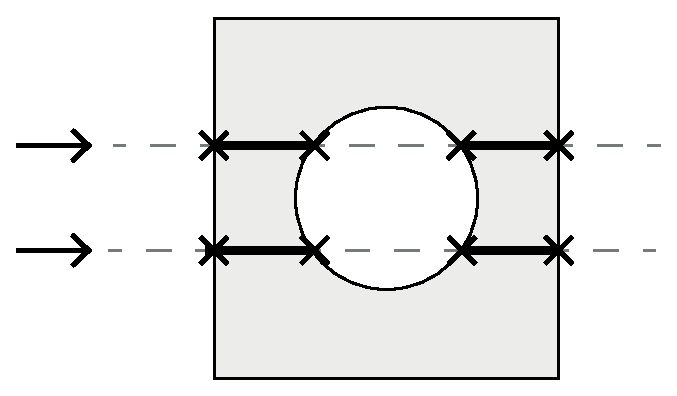
\includegraphics[width=\textwidth]{sections/methodology/figures/solid-watertight}
        \caption{Watertight 3D model cross section.}
        \label{fig:filling-watertight-model}
    \end{subfigure}
       \caption{Solid (voxelization) filling of 3D model cross section.}
       \label{fig:filling-3d-model}
\end{figure}


\section{Color system}
Asd

\section{GUI}


\break
\section{Design and modelling}
This section contains a description of the alternatives considered for designing...


\section{Plattform cross compatibility}
Mainly voxelizer-desktop program....??

\section{Building}
Id fugiat et ut veniam do anim anim labore dolor eiusmod eiusmod ex sit pariatur. Sit culpa nulla do aute. Eiusmod est enim do in in velit excepteur nulla id nostrud esse ipsum ipsum exercitation. Elit excepteur sint ad exercitation eiusmod exercitation fugiat. Magna laboris proident nisi aliqua sit cillum non velit est. Id commodo in culpa est ad irure officia velit duis.

\begin{figure}[h]
    \setlength{\abovecaptionskip}{25pt}
    \centering
    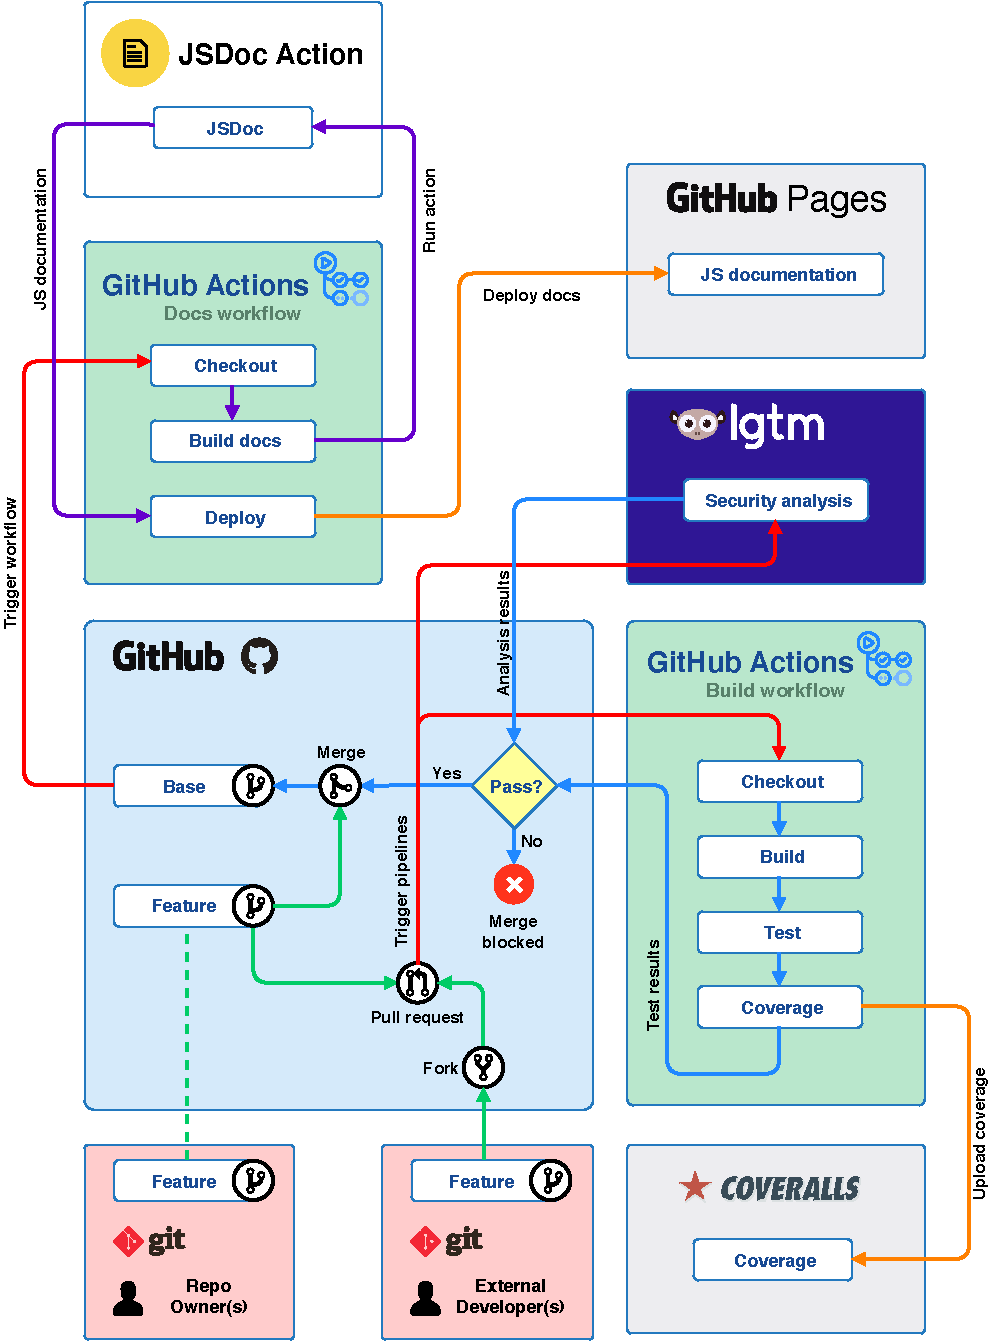
\includegraphics[page=1,scale=1]{sections/methodology/figures/pipelines.pdf}
    \caption{CI/CD pipelines}
    \label{fig:cicd-pipelines}
\end{figure}
\clearpage

Tempor esse exercitation est sunt eiusmod ea occaecat laboris exercitation et in. Officia amet sit nulla sit. Cillum sint consequat labore adipisicing aliqua laborum pariatur magna tempor adipisicing mollit qui voluptate.

\begin{figure}[h]
    \setlength{\abovecaptionskip}{25pt}
    \centering
    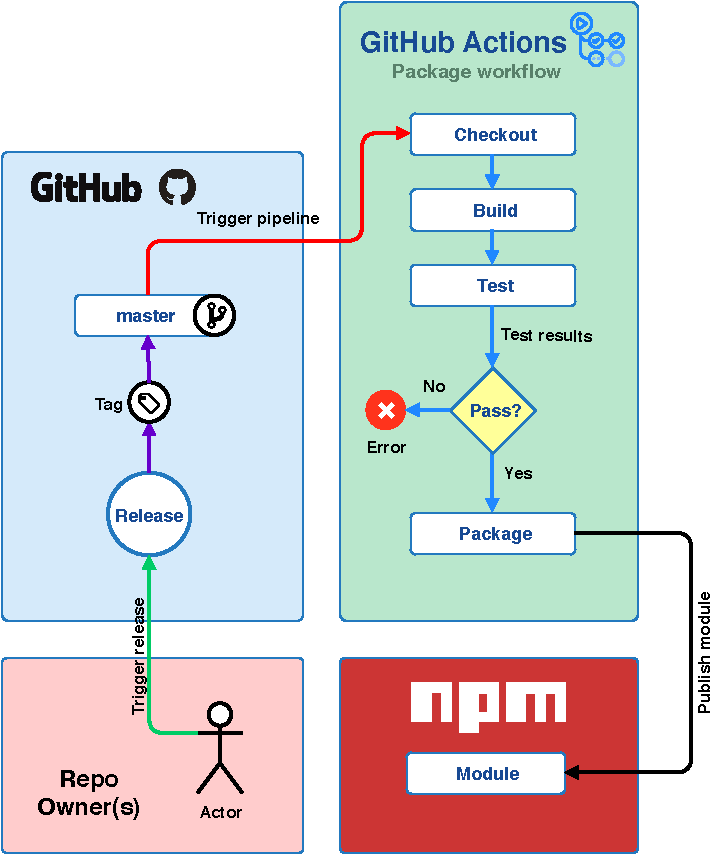
\includegraphics[page=1,scale=1]{sections/methodology/figures/release-automation.pdf}
    \caption{Automation of release publishing process.}
    \label{fig:release-automation}
\end{figure}

Aliquip proident sint laborum proident magna ut proident. Lorem irure laboris laboris in id adipisicing eiusmod ex. Mollit culpa commodo dolore enim. Ipsum sit aliqua nostrud cupidatat. Sit magna adipisicing sit adipisicing quis in magna nulla reprehenderit est quis incididunt. Eu reprehenderit ex dolore aliquip esse mollit nulla aute officia ea sit non culpa.